\begin{align*}
    pV &= K_{B}NT \comment{Ideal gas law}\\
    pV &= nRT
\end{align*}

\begin{equation*}
    \bar{E}_{\text{kin}} = \frac{1}{2} f N K_{B}T \comment{Equipartition thm}
\end{equation*}

\begin{equation*}
    \Delta U = Q + W \comment{1st Law}
\end{equation*}

\begin{equation*}
    \frac{Q}{\Delta T} = \alpha A \d{T}{x}
\end{equation*}

\begin{equation*}
    \ln(A!) \approx A\ln(A) - A \comment{Stirling approx.}
\end{equation*}

\begin{equation*}
    \Omega(N, q) = \frac{(q + N - 1)!}{q!(N - 1)!} \comment{Einstein solid}
\end{equation*}

\begin{equation*}
    \Omega(N, N_{\uparrow}) = \frac{N!}{N_{\uparrow}(N - N_{\uparrow})!} \comment{paramagnet}
\end{equation*}

\begin{equation*}
    S = K_{B} \ln \Omega \comment{entropy}
\end{equation*}

\begin{equation*}
    S(U,V,N) = K_{B}N \left[ \ln \left( \frac{V}{N} \left( \frac{4\pi m U}{3\hbar^{2} N} \right)^{\frac{3}{2}}  \right) + \frac{5}{2} \right] \comment{Sackur-Tetrode}
\end{equation*}

\begin{equation*}
    \frac{1}{T} \equiv \left[ \pd{S}{U} \right]_{N,V}
\end{equation*}

\begin{equation*}
    p \equiv T\left[ \pd{S}{U} \right]_{U,N}
\end{equation*}

\begin{equation*}
    \eta \equiv \frac{W}{Q_H} \comment{efficiency}
\end{equation*}

\begin{align*}
    H &\equiv  U + pV \\
    F &\equiv U - TS \\
    G &\equiv H - TS
\end{align*}

\begin{figure}
    \centering
    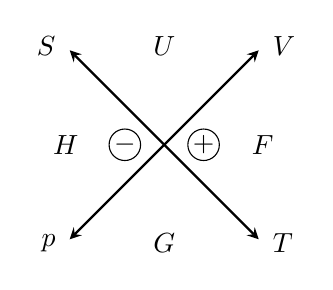
\begin{tikzpicture}[
        scale=0.5,
        trans/.style={thick,<->,shorten >=2pt,shorten <=2pt,>=stealth}
    ]
    \draw[trans] (0,0) node[below, left] {$p$} -- (5,5) node[above, right] {$V$};
    \draw[trans] (5,0) node[below, right] {$T$} -- (0,5) node[above, left] {$S$};
    \draw(0,2.5) node {$H$};
    \draw(2.5,0) node {$G$};
    \draw(5,2.5) node {$F$};
    \draw(2.5,5) node {$U$};
    \draw(1.5,2.5) node {$-$};
    \draw(1.5,2.5) circle(0.4);
    \draw(3.5,2.5) node {$+$};
    \draw(3.5,2.5) circle(0.4);
    \end{tikzpicture}
\end{figure}

\begin{align}
    \mathrm{d}U &= T\mathrm{d}S - p\mathrm{d}V + \mu \mathrm{d}N \\
    \mathrm{d}F &= -S\mathrm{d}T - p\mathrm{d}V + \mu \mathrm{d}N \\
    \mathrm{d}G &= -S\mathrm{d}T + V\mathrm{d}p + \mu \mathrm{d}N \\
    \mathrm{d}H &= T\mathrm{d}S + V\mathrm{d}p + \mu \mathrm{d}N
\end{align}



\begin{equation*}
    \d{p}{T} = \frac{L/T}{\Delta V} \comment{Clausius-Clapeyron relation}
\end{equation*}

\begin{equation*}
    \left(p + a\frac{N^2}{V^{2}}\right) \left(V - bN\right) = K_{B}NT \comment{Van der Waals eqn}
\end{equation*}

\begin{equation*}
    P(S) = \frac{1}{z} \exp \left(- \frac{E(s)}{T} \right)
\end{equation*}

\begin{equation*}
    z = \sum_{s} d(s) \exp \left(- \frac{E(s)}{T} \right)
\end{equation*}

\begin{equation*}
    \langle E \rangle = -\pd{\beta} \ln z
\end{equation*}

\begin{equation*}
    F = - T \ln z
\end{equation*}

\begin{equation*}
    p(s) = \frac{1}{\mathcal{Z}} \sum_{s} \exp \left(- \frac{E(s) - \mu N(s)}{T} \right)\end{equation*}

\begin{equation*}
    \mathcal{Z}(T,V,\mu) = \sum_{s} \exp \left(- \frac{E(s) - \mu N(s)}{T} \right)
\end{equation*}
